\section{Method Overview} \label{sec:workflow}

With an objective to compute a well-connected midsurface, the input model undergoes through transformations as shown in Figure \ref{fig_sysarch} and Algorithm \ref{alg_FBDMidsurf}. 

\begin{itemize}[noitemsep,topsep=2pt,parsep=2pt,partopsep=2pt,leftmargin=*]
\item \textbf{Input}: The input to the overall system is a feature-based CAD model, represented by  ($\cup_qf^3$), where `$\cup$' denotes a collection, of `$q$' features (`$f$') having dimensionality `$3$' (solids). In practice, the thin-walled CAD models exist in various representations/formats/types, such as mesh, solid, feature-based CAD, etc. This research, as it leverages feature information, expects a feature-based CAD model as the input. 
\todo[backgroundcolor=yellow]{\textbf{Reviewer}:  A limitation of the
approach is that the starting point for the midsurface generation is a feature based CAD model which may not
always be available. Provide a more detailed discussion of the potential limitations of using a feature model as the starting point
for the process and how these limitations can be overcome. This is particularly problematic because each CAD system uses its own feature
definitions and the feature translation to "sweep" operators will therefore be different for each CAD package. \\ \textbf{Author}: Mentioned the limitations }This, at times can be deemed as a  limitation, in case of unavailability due to format restrictions, proprietary data, etc. But, techniques such as segmentation, cellular decomposition, feature recognition (FR), etc. can be used effectively to convert the non-feature-based model to a feature-based one.
\end{itemize}
\todo[backgroundcolor=yellow]{\textbf{Reviewer}: They mention that the input
model can be a solid (B Rep or CSG) or a mesh or feature­based. Then, they refer to segmentation,
decomposition or feature recognition but these processes are highly interactive and, later on in the paper,
there no more information about the new issues related to these processes. As such, there is no need to
mention them if nothing is demonstrated and analyzed with their processing, which is the present case. \\ \textbf{Author}: Removed the portions}

\todo[backgroundcolor=yellow]{\textbf{Reviewer}:  On p7 reference the sources which explain translation from Brep to feature based cad model  \\ \textbf{Author}:Removed the mention}

%\bigskip
%
%\begin{minipage}[c]{\linewidth}
%    \begin{minipage}[c]{0.59\linewidth}
\begin{itemize}[noitemsep,topsep=2pt,parsep=2pt,partopsep=2pt,leftmargin=*]
\item \textbf{Defeaturing}: Computes the gross shape by removing irrelevant features. Defeatured model  is denoted as ($\cup_rf^3, r \leq q$)  (Section \ref{sec:defeaturing}, \cite{YogeshCADConf2015}). %%%%%%%%%% ADD (\cite{YogeshCADConf2015}) in NON DOUBLE BLIND PAPER

\item \textbf{Generalization/Abstraction}: As mentioned in Section \ref{sec:facepairdetection}, ``ABEL'' transforms variety of form-features into ``Loft'' ($L$). The model thus becomes ($\cup_rL^3$) (Section \ref{sec:abstraction}, \cite{YogeshIITG2014}). %%%%%%%%%%% ADD  (\cite{YogeshIITG2014}) LATER

\item \textbf{Decomposition}: Cellular decomposition is performed at each feature step to form non-volumetrically-overlapping cellular bodies having respective owner-Lofts. A graph is populated with the cellular bodies at the graph-nodes (Section \ref{sec:decomposition}).

\item \textbf{Midsurface Computation}: Using topology of the graph, the nodes are classified into solid cells ($sCell$s) and interaction-resolving nodes (interface cells, $iCell$s).  $sCell$s generate midsurface patches and $iCell$s connect them (Section \ref{sec:midsurface}).

\item \textbf{Validation}:  Midsurface needs to faithfully mimic the parent shape. A topological method is proposed and used to validate correctness of the midsurface (Section \ref{sec:validation},  \cite{YogeshCADandA2015}).

\item  \textbf{Midsurface/Output}: A well-connected midsurface is then sent to downstream applications such as CAE analysis.  
\end{itemize}

%    \end{minipage}
%    \hfill
%    \begin{minipage}[c]{0.38\linewidth}
\begin{figure}[h!]
\centering  
	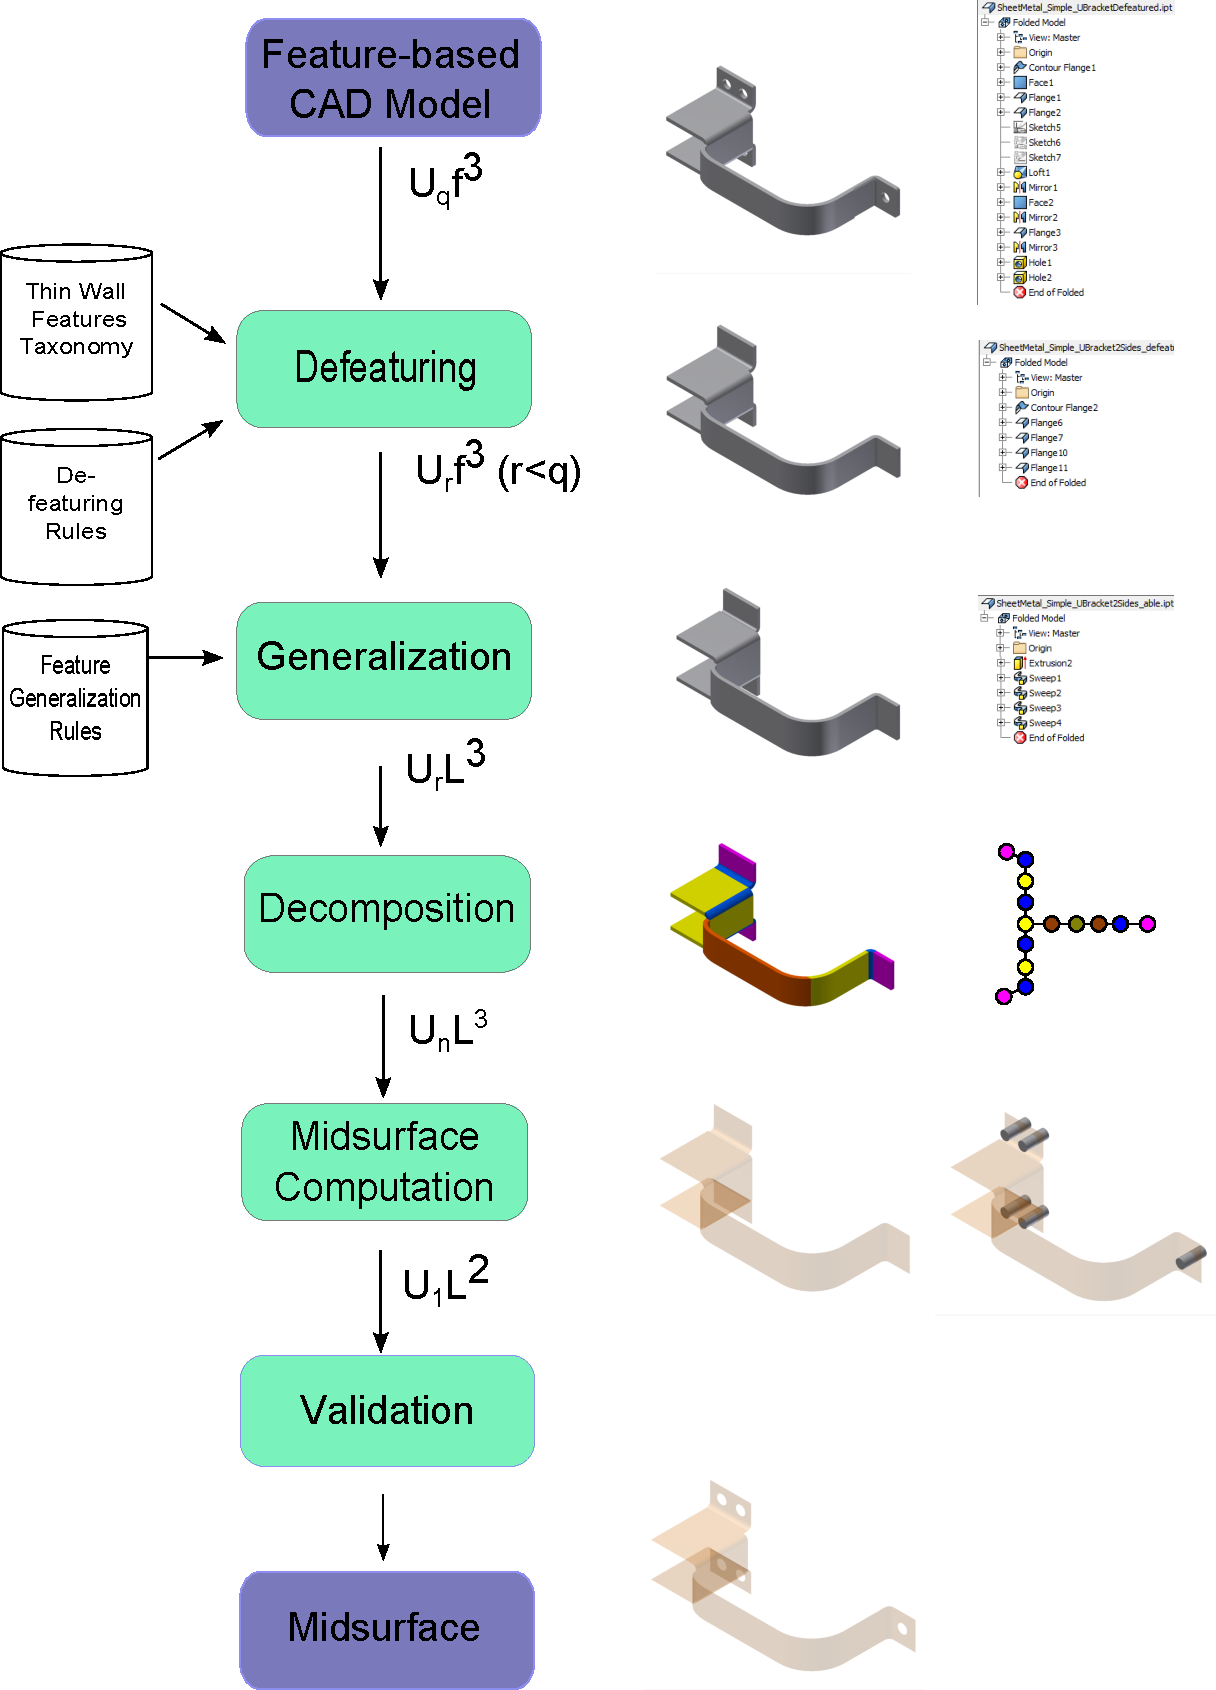
\includegraphics[width=0.85\linewidth]{../Common/images/SystemArchitecture3.pdf}
	%\captionof{figure}{Overall work-flow }
	\caption{Overall work-flow }
	\label{fig_sysarch}
	\end{figure}

%    \end{minipage}
%
%\end{minipage}    

	\todo[backgroundcolor=yellow]{\textbf{Reviewer}:   Change diagram to show that number of cells, say,q, are far more than `n', \\ \textbf{Author}: Changed Architecture diagram}
	
\bigskip

\begin{algorithm}[!h]
\caption{Feature-based midsurface computation}
\label{alg_FBDMidsurf}
\begin{algorithmic}
	\REQUIRE Feature-based CAD model  represented by  ($\cup_qf^3$)
	\STATE $\cup_rf^3 = feature\_based\_defeaturing(\cup_qf^3)$, where, $r \leq q$
	\STATE $\cup_rL^3 = feature\_based\_generalization(\cup_rf^3 )$
	\STATE $\cup_nC^3 =feature\_based\_cellular\_decomposition(\cup_rL^3)$, where, $C_i \cap C_j = 0| O_{i,j}^2$
	\STATE $G(n, ) = compute\_graph\_nodes(\cup_nC^3)$
	\STATE $(Gn,e) = find\_overlaps\_generate\_edges(G(n, ))$
	\STATE $(sCell,iCell) = categorize\_cells((Gn,e))$
%	\IF{ $n_i\rightarrow edges > 2$ \& \ $n_i \rightarrow body \rightarrow is\_thin = true$ \& $O_{i,j}^2$ are adjacent} 
%		\STATE $type(n_i) = iCell$ 
%	\ELSE
%		\STATE $type(n_i) = sCell$
%	\ENDIF
	\FORALL{$sCell$}
		\STATE $\cup_vL^2 = compute\_midsurface\_patch(sCell)$ (Algorithm \ref{alg_MidsurfsCell})
	\ENDFOR
	\FORALL{$iCell$}
		\STATE $\cup_wL^2 = resolve\_interactions(iCell)$ (Algorithm \ref{alg_MidsurfiCell})
	\ENDFOR
	\RETURN $\cup_1L^2 = (\cup_vL^2) \cup (\cup_wL^2)$

\end{algorithmic}
\end{algorithm}

\bigskip

Following sections provide details of each of the above-mentioned modules.

\subsection{Defeaturing} \label{sec:defeaturing}
Defeaturing means removal of unwanted features (\cite{Thakur2009}). It has been observed that a simplified shape, representing the overall shape, called ``gross shape'', yields an effective midsurface (\cite{YogeshCADConf2015}). Thus, the objective of this defeaturing module is to compute the gross shape by removing irrelevant features. The selection/eligibility of the irrelevant features is decided by two proposed approaches. In the first, sheet metal domain-specific features (being one of the major class of thin-walled models) are removed based on irrelevance. In the second, relative size of the remnant volumes (and not the full volumes) of features decided their eligibility for removal. Both phases can be customized. Phase I can be customized for different domains-specific eligibilities and Phase II can be customized with different size-threshold values (\cite{YogeshCADConf2015}).

\todo[backgroundcolor=yellow]{\textbf{Reviewer}:  Be more precise to characterize the shape transformations that take place in this step. Explain gist of the work, steps etc. Once the input model is defeatured, the authors state that its number of features has decreased. This is
rather obvious. What is the key here are the corresponding shape constraints set on the resulting solid, i.e.
what happens if the resulting solid has not an appropriate morphology for idealization in some areas? The
authors refer to a defeaturing engine of sheet metal feature: does this mean that they consider parts with a
constant thickness, which is consistent with comments on Table 1 but this is not bringing new contribution
compared to prior work of Armstrong et al. or Boussuge et al. \\ \textbf{Author}: Added more details}

In addition, a novel idea of caching bodies of large/relevant negative features is used.  Features, like Holes and Cuts if by usual rules do not get suppressed, they are still suppressed and their respective tool-bodies are preserved. These bodies, called ``Dormant bodies'', are then used in the last stage, to pierce the final midsurface. With this arrangement, computing midsurface patches is simplified due to lack of holes, while re-piercing of the cached dormant bodies ensures their faithful representation back in the midsurface.

\subsection{Abstraction/Generalization}\label{sec:abstraction}
Features not only carry shape information such as geometry and topology but also embed meta-information based on the application context (\cite{Shah1995}). With a variety of applications, each having its own need,  has resulted into various feature-schemes not only in different CAD applications, but also in various environments present within the same CAD application.  This causes a plethora of cases to deal with for writing a feature-based algorithm. Abstraction alleviates this problem by the extraction of a generic feature-form.  In the context of current research, it indicates the  finding of a generic feature, which will represent most of the available features. In the Generalization/Abstraction module, input feature tree is converted into a Loft-feature tree \footnote{Extrude, Revolve and Sweep are considered as variations of Loft \cite{YogeshIITG2014}. Sweep has a single profile and a singe guide curve, whereas Loft can have multiple profiles and a guide curve. In the context of current research, which is focused on sheet metal parts having constant thickness, Sweep with a single profile and a guide curve is sufficient to represent most of the features.} and sent for Midsurface computation. 

\todo[inline, backgroundcolor=yellow]{\textbf{Reviewer}:  It is important to show the effect of the conversion with the effective decomposition of the solid into
different subsets for the normal feature tree as well as the ABEL feature tree. At present time, the figure
does not bring much information.\\ \textbf{Author}: Removed the Normal-toABEL tree conversion figure altogether. ABEL and Decomposition are explained bit more}

\todo[inline, backgroundcolor=yellow]{\textbf{Reviewer}:  Then, when applying the generalization process of ABEL, it must be clearly stated that this process is user­
assisted and it lacks of arguments and description to show how robust it is, considering that its efficiency is
a key issue to the proposed method. Give more details from the paper\\ \textbf{Author} : Its an automatic transformation. Not sure what is to with efficiency as such. Once rules are in place, conversion to Loft should happen fine}

\todo[backgroundcolor=yellow]{\textbf{Reviewer}:  The referenced paper about the generalization of features, which is also a conference paper of the authors,
is not enough to reproduce the result of the method. .\\ \textbf{Author}:  More detailed elaborations are needed.}

\subsection{Validation}
\label{sec:validation}

Midsurface is expected to truly represent the input model, both in terms of geometry and topology. It is tedious to follow the manual process of inspection to validate it, especially for the complex models.  Current methods use Hausdorff's distance measure to verify geometric correctness but there are no established methods to ascertain topological correctness (similar connection configuration compared to the input).  The main idea behind the proposed formulation is that, the generated midsurface is expected to be such that it is obtained as if the solid body is shrunk to its overall neutral plane. As a reverse validation, if such a midsurface is thickened, it should represent a solid body as close to the original solid as possible. The solid's topological validity is then checked using the Euler-Poincar\'e's manifold equation. If the original midsurface had any gaps or overlaps, the resultant solid will not satisfy the same valid manifold condition. 
 (\cite{YogeshCADandA2015}). 

\todo[backgroundcolor=yellow]{\textbf{Reviewer}:  In section 2.4 explain more clearly the basis for FBCD which is the starting point for your method (this is
currently done to some extent on p10 but it should be at the beginning of the method section \\ \textbf{Author}: Moved Overall algo in the beginning}
\todo[backgroundcolor=yellow]{\textbf{Reviewer}: The resulting approach is presented as automatic, which does not let the user adapt connection under
different mechanical criteria. This is restrictive. \\ \textbf{Author}: Don't know what to do here. Mechanical criterion means Load and boundary conditions, SO they are not taken into account}

\bigskip
Following sections focus on the remaining parts of the work-flow: Decomposition and Midsurface Computation.

\todo[backgroundcolor= yellow]{Reviewer:  The methodology presented in the paper is quite difficult to follow because much of the background theory is
found in the other papers by the author, or other references. The authors need to articulate much more clearly
the basis for their method and how it differs to previous work. \\ Author: Added relevant details in places.}


\section{Decomposition}
\label{sec:decomposition}

As mentioned in Section \ref{sec:workflow} our approach starts with a feature-based CAD model. The model is defeatured by applying a set of strategies so that the output CAD model has small or irrelevant features removed. The feature tree of defeatured CAD model is transformed to  Loft-feature-tree . Now the advantage is that, the computation logic of midsurface patches needs to be based on only the ``Loft'' feature, that is, profile(s) and a guide curve (Algorithm \ref{alg_MidsurfsCell}). But in such a part, each Loft feature is not a separate entity but is booleaned at each tree-node to the existing model till that state. Detecting and separating the common portions will be needed to decide on the midsurface generating sub-volumes and patch joining sub-volumes. This splitting is done by Decomposition.
\todo[backgroundcolor=yellow]{\textbf{Reviewer}: The authors distinguish the Sweep features from the Loft one ,here, they use
the same designation. It is no longer clear what the difference is between these features. Change the picture to make all SWEEPs or make SWEEP/LOFT. State the different between two and use of interchangeability here. \\ \textbf{Author}: Added clarification footnote}
%Feature based CAD model is decomposed by the process of feature-based cellular decomposition (FBCD) in which the feature volumes are partitioned into cell-bodies.
%Features with cellular structures are found in the research by Bidarra, Chen, etc. \cite{Bidarra1993,BidarraKrakerBronsvoort1998, Chen2006} whereas cellular decomposition and their feature recognition can be found in works of Woo2013,Boussuge2013a,Wu2014,Woo2014}).  Most cellular decomposition methods work on the final soilid shape represented by B-rep (Boundary Repreentation) and use convex partitioning useful to build algorithms found in simplification \cite{JaeLee2004, SangHunLee2005}, Computer-Aided Manufacturing (CAM), etc. \cite{Woo2002}
\todo[backgroundcolor=yellow]{\textbf{Reviewer}:  However, this important process, though part of authors' prior work must be
clarified enough to understand how the solid is segmented and how this is achieved, i.e. interactively or
automatically, how robust is it? This is critical since the authors claim a divide and conquer approach and
this decomposition is the divide criterion. As such,  the divide phase description is entirely missing. \\ \textbf{Author}: Removed the original mention altogether}
\todo[inline,backgroundcolor=yellow]{\textbf{Reviewer}:  Subsequently, the authors refer to a cellular decomposition but they don't explicitly state what are the cells
and what are the constraints of this decomposition and how there are automatically satisfied though it seems
that it can fail because the authors refer to minimum failure but this process cannot be evaluated. \\ \textbf{Author}: Added decomposition criterion, pluses minuses etc}
This work uses cellular decomposition in the context of feature-based CAD model (FBCD) with primary rules as:
\begin{itemize}[noitemsep,topsep=2pt,parsep=2pt,partopsep=2pt]
\item \textbf{Feature partitioning}: Internal as well as external booleans  are changed to the ``New Body'' type, so that the tool-body volumes get separated. The volumes may still overlap with each other.
\item \textbf{Concave edge partitioning (CEP)}: Overlapping volumes are split at concave edges. Faces at these edges are extended and used as partitions to split. In this work, extensions are not done infinitely (or covering the part's bounding box) but within the influence zone decided by two interacting features.
\end{itemize}

\todo[backgroundcolor=yellow]{\textbf{Reviewer}: The cellular decomposition method implemented in this paper is very unclear. The authors just mentioned
several existing celluar decomposition methods but not the specific one that they used. For example, I do
not understand how the authors generated the cellular model in Fig. 10(b) and (c). To my knowledge, I haven't
seen such a celluar decomposition shown in the figure. Which faces do you extend to generate the cellular
model? How do you decompose the portions having tangent edges? Authors need to explain the process of
cellular decomposition in more detail. \\ \textbf{Author}: Decomposition rules and figure \ref{fig_fbcd} added}
%
%\begin{figure}[!h]
%\centering     %%% not \center
%\subfloat[Before decomposition]{\label{fig_twofeat}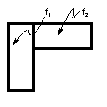
\includegraphics[width=0.25\linewidth,valign=t]{../Common/images/FeatureInteractionPart.pdf}}
%\subfloat[After decomposition]{\label{fig_featinteract}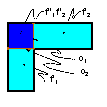
\includegraphics[width=0.25\linewidth,valign=t]{../Common/images//FeatureInteractionCells.pdf}}
%\caption{ Feature-based cellular decomposition}
%\label{fig_fbcd}
%\end{figure}

\todo[backgroundcolor=yellow]{\textbf{Reviewer}: In particular, this constraint has a direct consequence
on the shape of the features obtained, hence on contours taken into account to be idealized whereas having
a possibility to have interpenetrating volumes can simplify these contours and ease idealization process for
each feature, eventually leaving the user adapt the connections between the sub­domains, which can be
handled mechanically. This improves the results as in the work of Boussuge et al. Therefore, the proposed
approach does not bring new insights. \\ \textbf{Author}: Did not follow the comment. Added clear distinction of our work wrt past works}

\begin{figure}[!h]
\centering     %%% not \center
\subfloat[Original Part]{\label{fig_beforecd}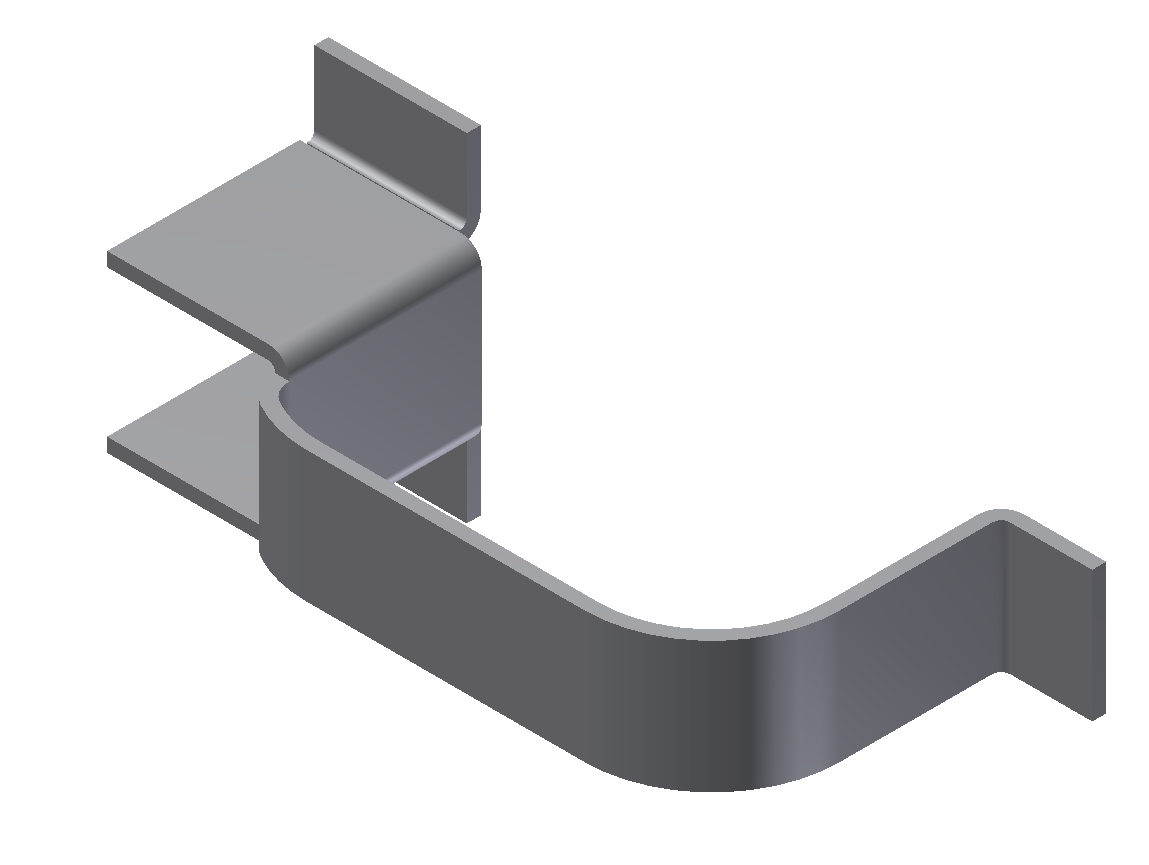
\includegraphics[width=0.26\linewidth,valign=t]{../Common/images/DecompBracketInput}}
\subfloat[Feature Partitioning]{\label{fig_cd}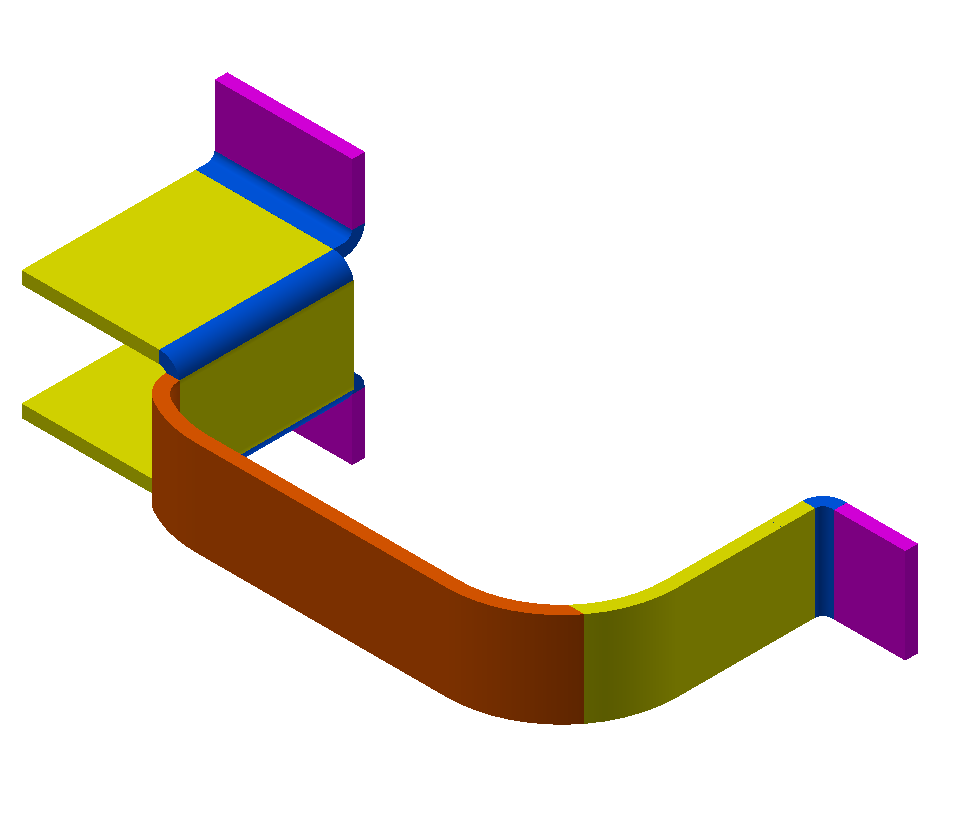
\includegraphics[width=0.223\linewidth,valign=t]{../Common/images/DecompositionBracketOutputPart}}\qquad
\subfloat[Overlapping Features]{\label{fig_twofeat}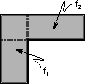
\includegraphics[width=0.19\linewidth,valign=t]{../Common/images/FeatureInteractionMergedPart.pdf}} \qquad
\subfloat[CEP]{\label{fig_featinteract}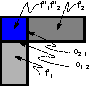
\includegraphics[width=0.19\linewidth,valign=t]{../Common/images//FeatureInteractionMergedCells.pdf}}
\caption{ Feature-based cellular decomposition}
\label{fig_fbcd}
\end{figure}

\todo[backgroundcolor=yellow]{\textbf{Reviewer}: The authors refer to redundant cell but this is not defined and, finally, they assume that their FBCD
generates a decomposition where each cell represents a correctly assigned owning­feature but there is no
demonstration showing it can be achieved. \\ \textbf{Author}: Decomposition rules and figure \ref{fig_fbcd} added}

Cells do not overlap volumetrically but can touch others at the boundary faces, only fully, but not partially.   Figure \ref{fig_beforecd} is the input model and Figure \ref{fig_cd} is the output of FBCD, with each cell-bodies shown in different colors. Figure \ref{fig_twofeat} shows a representative case schematically, where two features $f_1$ and $f_2$ are interacting. Interaction can have full/partial volumetric/surface overlaps. Typical cellular decomposition happens at the concave edges. In the above scenario, volumes of $f_1$ and $f_2$ are partitioned in such a way that a common cell (with owner $f''_1f''_2$) is formed (Figure \ref{fig_featinteract}). Remaining portion of $f_1$ and $f_2$ are termed as $f'_1$ and $f'_2$ respectively.  Overlapping faces are denoted as $O_1$ and $O_2$, where $O$ denotes ``Overlapp'' and $_1$ and $_2$ are the instances. Thus, now, the cell-bodies do not overlap volumetrically [$O_{i,j}^3 = 0$] (meaning, Overlap between bodies $_i$ and $_j$ which is of dimensions $^3$, that is, volumetric), but may overlap at faces [$O_{i,j}^2$] (meaning, Overlap between bodies $_i$ and $_j$ which is of dimensions $^2$, that is, surface-wise) fully and not partially, denoted as [ $C_i \cap C_j = 0| O_{i,j}^2$] (meaning, Intersection $\cap$ of cells $C_i$ and $C_j$ is either nothing or full-surface, but not partial).

\todo[backgroundcolor=yellow]{\textbf{Reviewer}: Authors use the notations $O_{i,j}^3$  and $O_{i,j}^2$ and  $C_i \cap C_j = 0| O_{i,j}^2$ but their meaning is not given. \\ \textbf{Author}: Added explanations }


\begin{figure}[!h]
\centering 
\begin{minipage}[h]{0.28\linewidth} 
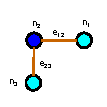
\includegraphics[width=0.8\linewidth]{../Common/images/FeatureInteractionGraph.pdf}
\end{minipage}
\begin{minipage}[h]{0.28\linewidth} 
\centering 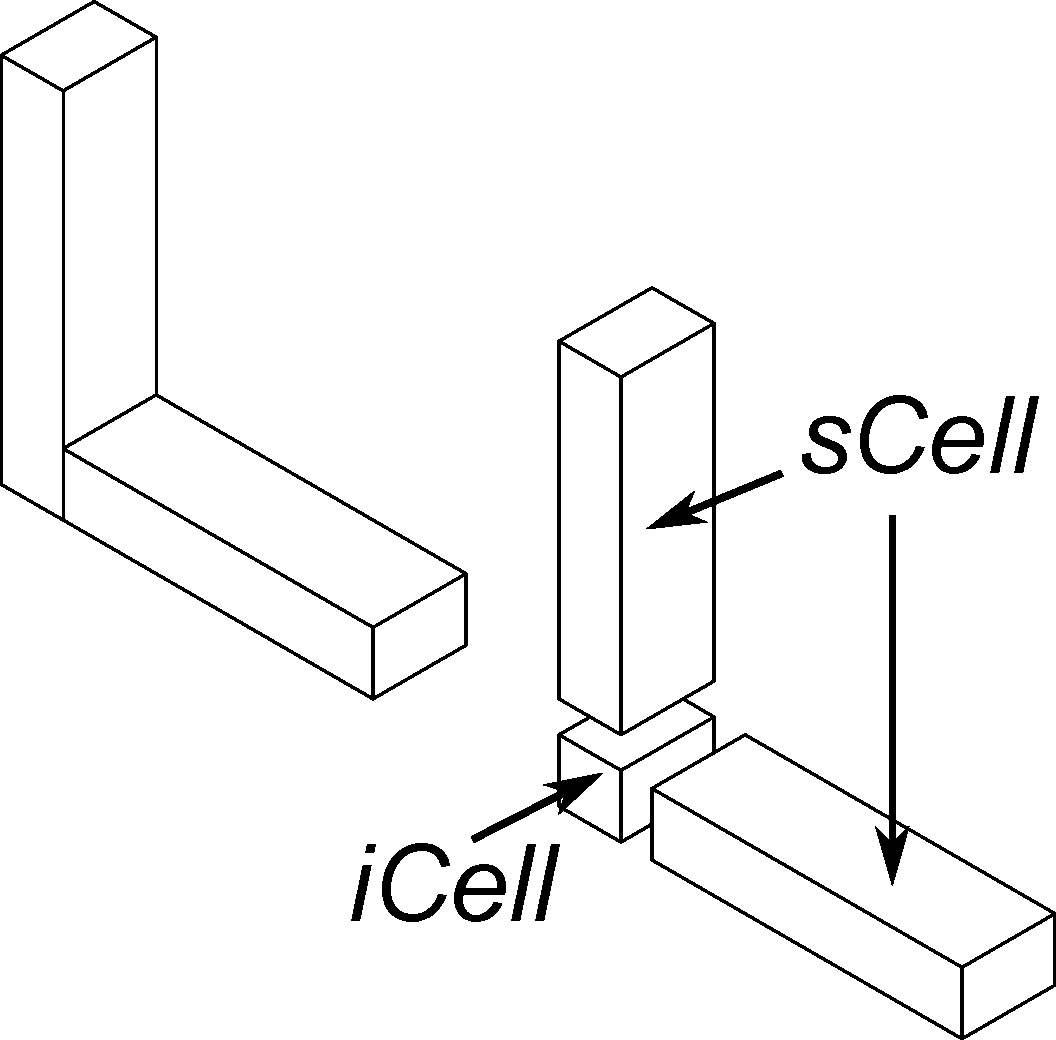
\includegraphics[width=0.7\linewidth]{../Common/images/CellDecompExample.pdf}
\end{minipage}
\begin{minipage}[h]{0.28\linewidth} 
\begin{itemize}[noitemsep,topsep=2pt,parsep=2pt,partopsep=2pt,label={}]
\item $n_1 = sCell_1= f'_1$
\item $n_2 = iCell_1 = f''_1f''_2$
\item $n_3 = sCell_2 = f'_2$
\item $e_{12} = O_1$
\item $e_{23}= O_2$
\end{itemize}
\end{minipage}
\caption{Feature-based Cellular Graph}
\label{fig_featgraph}
\end{figure}

\todo[backgroundcolor=yellow]{\textbf{Reviewer}:  It has also to be noted that the example of fig. 6 ??? produces n>m, which contradicts the work flow described in sec. 2.3 \\ \textbf{Author}: Could not follow the comment. Probably a misunderstanding. Changed $n$ to some other letter, as it was used as number of features in architecture diagram}


FBCD results in $n$ cell-bodies, each assigned with a Loft owner-feature. A cell adjacency graph [CAG, $G(n,e)$] is formed with the $n$ nodes, each representing a cell-body. Each face-overlap between two nodes is represented by an edge ($e$).  Figure \ref{fig_featgraph} shows the CAG of simple cell bodies configuration of a ``L'' shaped part. Node $n_1$ corresponds to a cell-body, with owning feature $f'_1$, whereas node $n_3$ corresponds to the cell-body with owning feature $f'_2$. The common cell-body owned by $ f''_1f''_2$ is represented by node $n_2$.  Edge $e_{12}$ corresponds to the overlapping face $O_1$, where as  Edge $e_{23}$ corresponds to the overlapping face $O_2$. 

Advantage of the CAG representation is that it is easier to classify nodes and delegate specific computational work to them.  Looking at the connectivity at each cell-nodes, they are classified into solid cells ($sCell$) and interface cells ($iCell$).  Generating midsurface patches is delegated to the $sCell$s  and the problem of resolving interaction amongst the midsurface patches is carried out by the $iCell$s. The classification strategy,  based on the simple graph-topology rules, simplifies the complexity of the midsurface generation problem to a great extent.  Thus, this work does not need to enumerate specific heuristic rules used for specific connection types, or underlying geometry types.  The following section \ref{sec:midsurface} details the technique. %The commonly-shared cells are marked as interface cells ($iCell$) and the others as solid cells ($sCell$)  



%
%\begin{figure}[h]
%\centering 
%\begin{minipage}[h]{0.48\linewidth} 
%\centering 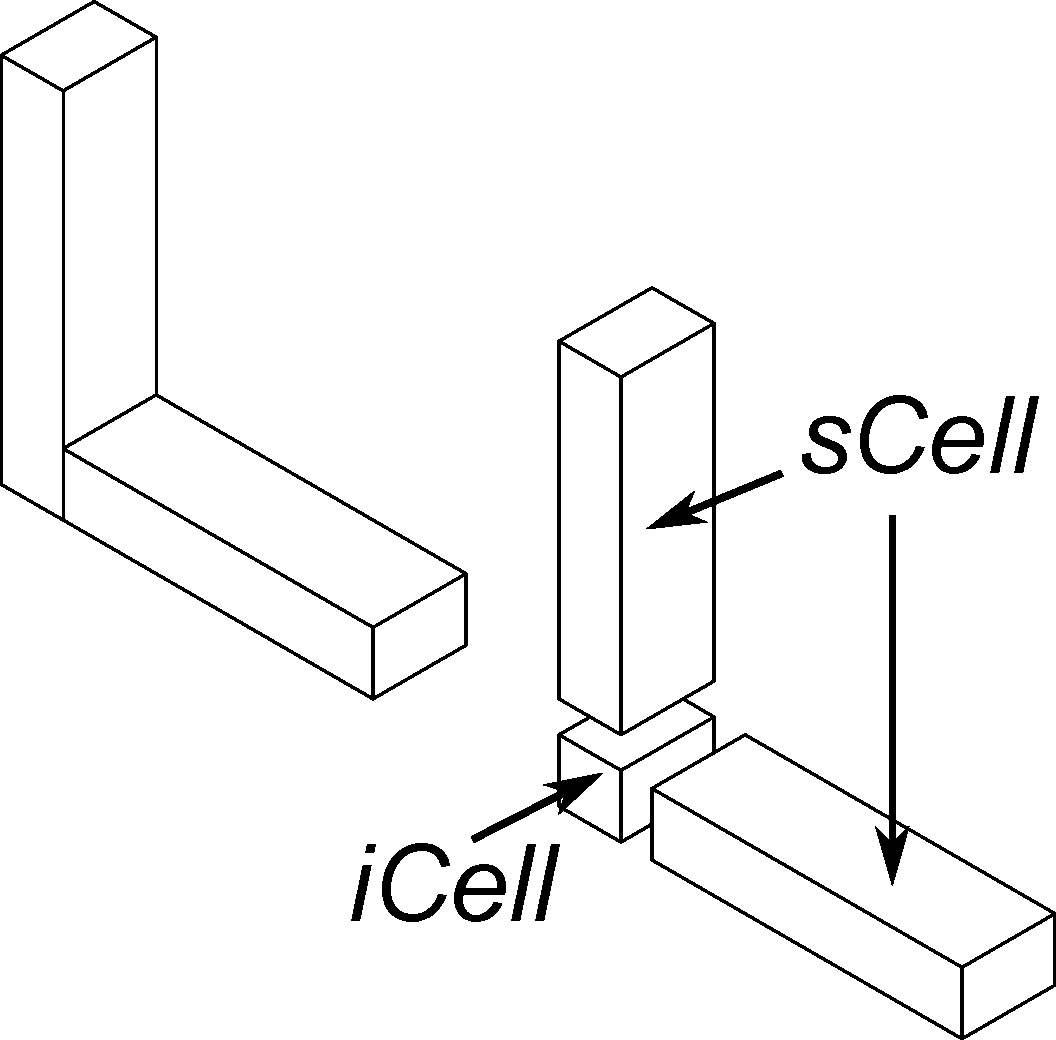
\includegraphics[width=0.7\linewidth]{../Common/images/CellDecompExample.pdf}
%\caption{Classification of Cells (\cite{Treeck})}
%\label{fig_celldecompexample}
%\end{minipage}
%\begin{minipage}[h]{0.48\linewidth} 
%\begin{mydef}
%Solid cell ($sCell$) is a node with 0 or 1 incident edge% any adjacent node with owning-feature as ``Loft'' and is not an $iCell$.
%\end{mydef}
%\begin{mydef}
%Interface cell ($iCell$) is a node with 2  or more incident edges %and has respective overlapping faces ($O_1,O_2$) adjacent to each other.
%\end{mydef}
%In Figure \ref{fig_featgraph},  $n_1$ and $n_3$ are solid cells ($sCell$), where as $n_2$ is an interaction cell ($iCell$).  $sCell$ are midsurface patch computing cells, which look at the $profile$ and $guide$ of the owning-feature to compute the midsurface patch. $iCell$ are interaction-resolving cells, connecting all the midsurface patches incident on it.
%\end{minipage}
%\end{figure}
%
%\bigskip

\todo[backgroundcolor=yellow]{\textbf{Reviewer}: On P11, definition 1, should it state that an interface cell is a node with ``2 or more'' incident edges? \\ \textbf{Author}: Done}
\todo[backgroundcolor=yellow]{\textbf{Reviewer}: On P11, definition 2 does not seem to be posed in the same syntax as definition 1 (should it say ``one
incident edge'')? \\ \textbf{Author}: Done}
\todo[backgroundcolor=yellow]{\textbf{Reviewer}: The explanation of the types of ``adjacent node'' on p13/14 is not very clear and should be improved \\ \textbf{Author}: Removed that mention from the definition. Its no more there in the implementation as well}

%\begin{mydef}
%Interface cell ($iCell$) is a node with more than 2 incident edges and has respective overlapping faces ($O_1,O_2$) adjacent to each other.
%\end{mydef}
%
%\begin{mydef}
%Solid cell ($iCell$) is any node which is not an $iCell$.
%\end{mydef}
%
%	\begin{figure} [!h]
%	\centering
%	\includegraphics[width=0.7\linewidth]{../Common/images/CellDecompExample}
%	\caption{Decomposition and Classification of Cells (\cite{Treeck})}
%	\label{fig_celldecompexample}
%	\end{figure}
				


\section{Midsurface Computation}
\label{sec:midsurface}

Each node in CAG represents a feature sub-volume, also known as cell-body. A cell body has three dimensions, the two sides of the aligned bounding box of the profile and the length of the guide curve (say, $d_1,d_2,d_3$).
%\begin{mydef}
%\label{def:thincell}
%A cell-body is considered as Thin, if only one dimension is less than the threshold-factor ($t$) times any of the other two dimensions ( $d_1 < t.d_2 \quad \&  \quad d_1 < t.d_3$)
%\end{mydef}
%
%\begin{mydef}
%\label{def:thickcell}
%A cell is considered as Thick, if its both minimum two dimensions are less than the threshold-factor ($t$) times of the maximum dimensions ( $d_1 < t.d_3 \quad \&  \quad d_2 < t.d_3$)
%\end{mydef}

Nodes are classified as $sCell$s and $iCell$s as per the following definitions:
\begin{mydef}
\label{def:scell}
Solid cell ($sCell$) is a cell-body with only one of its dimensions ($d_1$) is less than the threshold-factor ($t$) times any of the other two dimensions ($d_2, d_3$), denoted as  $d_1 < t.d_2 \quad \&  \quad d_1 < t.d_3$. %node representing a Thin cell-body and with 0/1 incident edge.% any adjacent node with owning-feature as ``Loft'' and is not an $iCell$.
\end{mydef}
\begin{mydef}
\label{def:icell}
Interface cell ($iCell$) is a cell-body with  both minimum two dimensions ($d_1,d_2$)  are less than the threshold-factor ($t$) times of the maximum dimensions ($d_3$), denoted as  $d_1 < t.d_3 \quad \&  \quad d_2 < t.d_3$. %node with 2/more incident edges. %and has respective overlapping faces ($O_1,O_2$) adjacent to each other.
\end{mydef}

In Figure \ref{fig_featgraph},  $n_1$ and $n_3$ are solid cells ($sCell$), where as $n_2$ is an interaction cell ($iCell$).  The $sCell$ computes the midsurface patches, whereas the  $iCell$ connects all the midsurface patches incident on them. Both process are detailed out in the sections below.
			


\subsection{Computing midsurface patches in $sCell$s}
\label{sec:scell}
 Algorithm \ref{alg_MidsurfsCell} describes the procedure of computing the midsurface patches in the $sCell$s. The CAG is traversed node-by-node and the Loft-owner feature information of each node is extracted. The midsurface patch computation strategy is dependent on whether it is `Thick' or `Thin', based on the relative size of Loft/Sweep's profile $p$ and the guide curve $g$  (Definition \ref{def:thinprofile}) (\cite{YogeshIITG2014}). %%%%%%%%%% ADD (\cite{YogeshIITG2014}) LATE

\begin{mydef}
\label{def:thinprofile}
The profile $p$ is considered thin, if its thickness size (characterized by the length of its shortest side) is less than the threshold-factor times the length of the guide curve $g$, otherwise considered as ``Thick''.
\end{mydef}

The `threshold' mentioned in the Definition \ref{def:thinprofile} is calculated by analyzing various sheet metal models and can be adjusted for better output. For example, `thinness' criterion used by Woo \cite{Woo2013}  is $\frac{min(L,H)}{d} > X, 1.2 \leq X \leq 3$ , where $L$ is length, $H$ is height and $d$ is thickness of the shape. This work uses threshold as $2$.
\todo[backgroundcolor=yellow]{\textbf{Reviewer}:  The authors give a definition of thin profile but there is no connection with the thinness
parameter stated in the introduction. Further, the perimeter of the sweep feature does not account for its
compatibility with a mid­surface generation, e.g., having g much longer than the perimeter of p does not
mean that p can be processed for a mid­surface, especially if p is a circle. Also, there may not be a unique
solution, e.g. in case of a cube cell, all it shared faces with other cells can produce the same result. It is not
clear whether this can produce a globally connected mid­surface. \\\textbf{Author}: Changed the definition \ref{def:thinprofile}}


Following are the strategies :% (Fig. \ref{fig_ablemids})
%For `Thick Profile' \ref{def:thinprofile}) the profile-face is offset, else (called `Thin Profile', definition \ref{def:thinprofile}) , midcurve of $p$ is swept along $g$ (Figure \ref{fig_ablemids}).
	\begin{itemize}[noitemsep,topsep=2pt,parsep=2pt,partopsep=2pt]
	\item\textbf{Thick profile}:  If the profile $p$ is thick, offset the profile-face $p$ upto half of $g$ so as to lie midway generating midsurface patch refereed to as $m^2$ ($2$ signifies dimensionality degree, that is, a surface)%( Figure \ref{fig_thick})% shows a big (shown colored) profile being larger than the guide curve (shown as small top edge), goes for the offset logic.
	\item \textbf{Thin profile}:  If the profile $p$ is thin, a midcurve ($m^1$) is computed from $p$ using approach presented in \cite{YogeshETES2014, YogeshIJCAET2017} and it  is swept using the guide curve $g$ to generate the midsurface patch $m^2$.% (Fig. \ref{fig_thin}).
	\end{itemize}
%
%	\begin{figure}[!h]
%	\centering     %%% not \center
%	\subfloat[Sweep feature]{\label{fig_thickthinpart}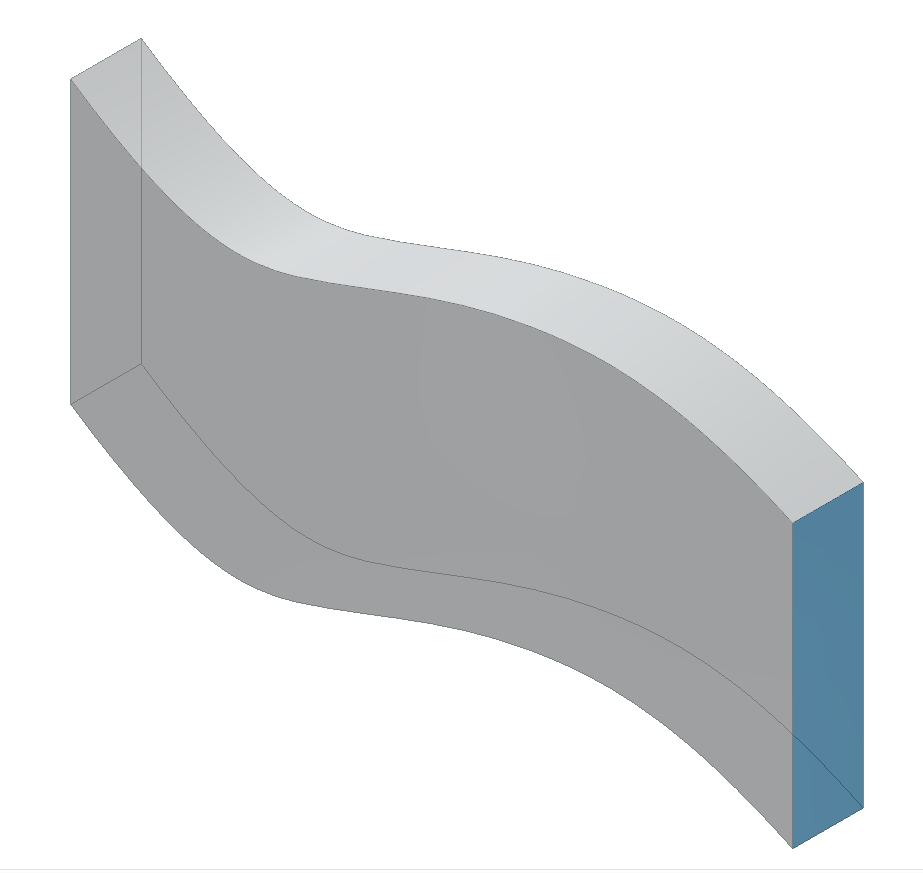
\includegraphics[width=0.26\linewidth,valign=t]{../Common/images/ThickThinProfilePartWireframe}}
%	\subfloat[Thick profile midsurface]{\label{fig_thick}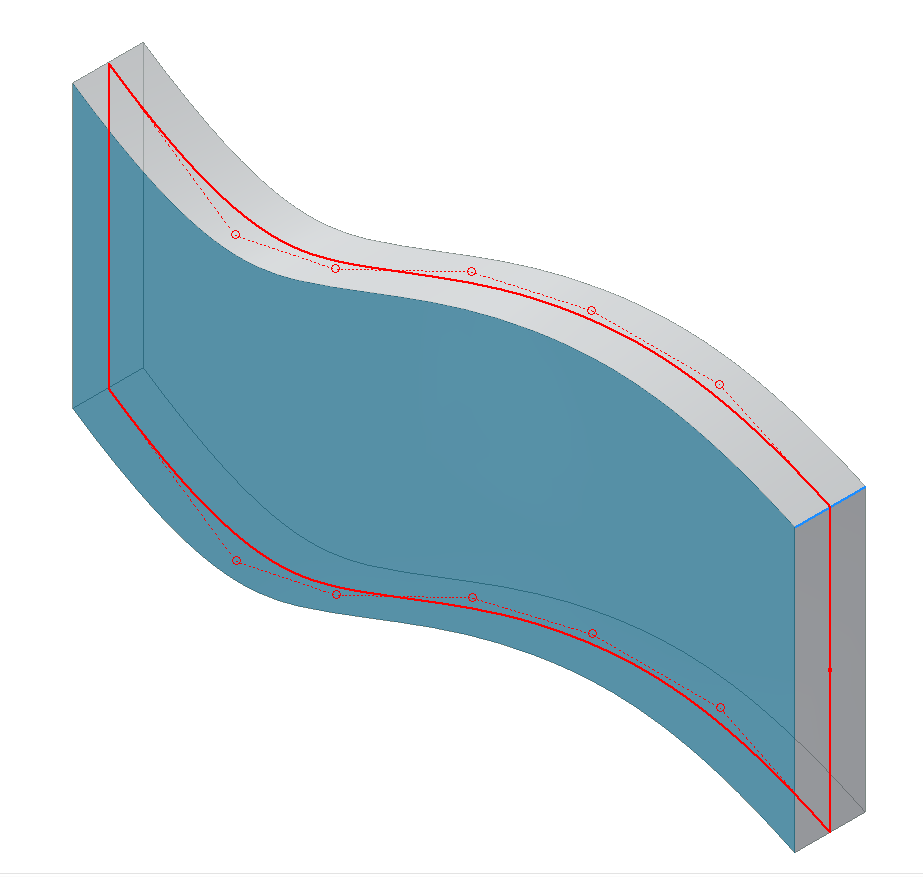
\includegraphics[width=0.26\linewidth,valign=t]{../Common/images/ThickProfileMidsurfWireframe}}
%	\subfloat[Thin profile midsurface]{\label{fig_thin}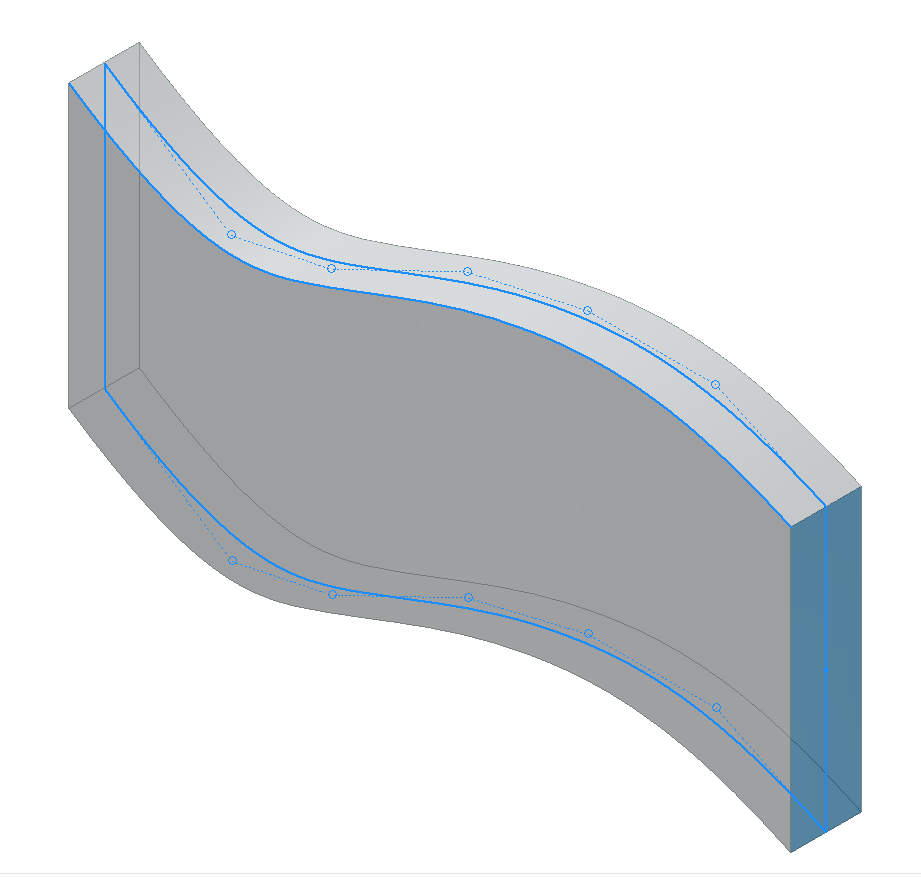
\includegraphics[width=0.26\linewidth,valign=t]{../Common/images/ThinProfileMidsurfWireframe}}
%%	\subfloat[Midsurface patches]{\label{fig_scells}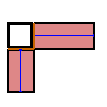
\includegraphics[width=0.23\linewidth,valign=t]{../Common/images/MidsurfPatches.pdf}}	
%	\caption{Midsurface based on relative size of Profile and Guide curve  (\cite{YogeshIITG2014}) } %%%%%%%% ADD (\{citeYogeshIITG2014}) LATER
%	\label{fig_ablemids}
%	\end{figure}

\todo[backgroundcolor=yellow]{\textbf{Reviewer}:   On P12, Figure 8, it is confusing to include Fig 8 (d) in the same figure as the other figures.  Also, the
orientation of the mid­surfaces in (b) and (c) are not very legible \\ \textbf{Author}: Done}

\begin{figure}[h]
\centering 
\begin{minipage}[h]{0.4\linewidth} 
\centering 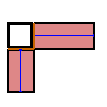
\includegraphics[width=0.65\linewidth]{../Common/images/MidsurfPatches.pdf}
\captionof{figure}{Midsurface patches in all $sCell$s}
\label{fig_scells}
\end{minipage}
\begin{minipage}[h]{0.55\linewidth} 
Applying these strategies for $sCell$s shown in Figure \ref{fig_fbcd}, the corresponding midsurface-patches generated are as shown in Figure \ref{fig_scells}.  Once all the $sCell$s are done with the computation of midsurface patches, the next step is to resolve interactions  between these patches in $iCell$s.
\end{minipage}
\end{figure}

\bigskip

	\begin{algorithm}[!h]
		\caption{sCell midsurface patch computation}
		\label{alg_MidsurfsCell}
		\begin{algorithmic}
			\REQUIRE $sCell$
			\ENSURE $size(sCell \rightarrow owning-feature(s)) = 1$
			\STATE $f = sCell \rightarrow owning\_feature()$
			\STATE $p = f \rightarrow get\_profile()$
			\STATE $g = f \rightarrow get\_guide\_curve()$
			%\STATE $is\_thin\_profile = \sqrt{Area(profile)} < threshold \times length(guide)$ 
			\IF{$is\_thin\_profile(p) == true$}
				\STATE $m^1 = p\rightarrow compute\_midcurve()$
				\STATE $m^2 = sweep(m^1 ,g)$
			\ELSE
				\STATE $m^2 = offset(p ,g/2)$
			\ENDIF
		\end{algorithmic}
	\end{algorithm}
	
	



\subsection{Resolving interactions between midsurface patches in $iCell$s}
\label{sec:icell}
Input to this module is a CAG with midsurface patches computed at all the $sCell$s. The sole responsibility of $iCell$s is to connect the midsurface patches incident on them, either by extending the midsurface-patches from the adjacent $sCell$s, or by generating new ones.  The CAG is used to traverse $iCell$s one by one. For each $iCell$, the midsurface patch interactions are resolved as follows (Algorithm \ref{alg_MidsurfiCell}) \footnote{Although the diagrams used to explain are simplistic/schematic, showing rectangular shapes with just two incident edges, the algorithm presented is applicable to a variety of shapes and more number of incident edges, as shown in Table \ref{tbl_fbcm}.}:

\def\myresolvecellcolumnwidth{0.3}
	\begin{figure}[!h]
	\centering     %%% not \center
	\subfloat[Expected adjustments]{\label{fig_icells}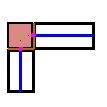
\includegraphics[width=\myresolvecellcolumnwidth\linewidth,valign=t]{../Common/images/MidsurfJoining.pdf}} \quad
	\subfloat[$sCell-iCell$ scenario]{\label{fig_sextensions}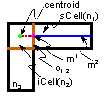
\includegraphics[width=\myresolvecellcolumnwidth\linewidth,valign=t]{../Common/images/sCellExtension.pdf}} \quad
	\subfloat[$iCell-iCell$ scenario]{\label{fig_iextensions}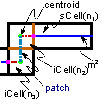
\includegraphics[width=\myresolvecellcolumnwidth\linewidth,valign=t]{../Common/images/iCellExtension.pdf}}	
	\caption{Resolving Interactions in the $iCell$}
	\label{fig_resolveiCell}
	\end{figure}
	
\todo[backgroundcolor=yellow]{\textbf{Reviewer}:   In Fig. 9, the authors give an example with
configs b and c, what about configs with a higher number of cells connected, 3, 4, …, p cells. It is not clear
how the connection algorithm will scale up. \\ \textbf{Author}: Added a footnote}

\bigskip
	
	\begin{algorithm}[!h]
		\caption{$iCell$ midsurface patch interaction resolution}
		\label{alg_MidsurfiCell}
		\begin{algorithmic}
			\REQUIRE $iCell$
			\WHILE{$size(iCell \rightarrow edges) > 0$}
				\STATE $e_i = iCell \rightarrow edge$
				\STATE $n_s = iCell $	
				\STATE $n_o = e_i \rightarrow get\_adjacent\_node(n_s) $			
				\IF{$n_o \rightarrow type == sCell$}
					\STATE $m_o = n_o \rightarrow query\_midsurface()$
					\STATE $O_f = e_i \rightarrow overlapping\_face()$
					\STATE $m^1 = surf\_surf\_intersection(O_f, m_o)$
					\STATE $m^2 = extrude(m^1, n_o \rightarrow centroid)$
				\ELSIF{$n_o \rightarrow type == iCell$}
					\STATE $c^1_1= get\_curve\_at\_centroid(n_s)$
					\STATE $c^1_2 = get\_curve\_at\_centroid(n_o)$
					\STATE $m^2 = create\_patch(c^1_1, c^1_2)$
					\ENDIF
			\ENDWHILE
		\end{algorithmic}
	\end{algorithm}

\bigskip
Each $iCell$ is connected with adjacent cells via edges $e$(s).  Each incident $e$ has two nodes (like $e_{12}$ has $n_1$ and $n_2$  in Figure \ref{fig_featgraph} ), where one is the ``self'', the current $iCell$ and the second one is called the ``adjacent node''.  The ``adjacent node'' could be either a $sCell$ or an $iCell$.  

If the ``adjacent node'' is a $sCell$, the adjacent midsurface-patch is extended up to $iCell$'s centroid (Fig. \ref{fig_sextensions}). An intersection curve ($m^1$) is computed between the overlapping face ($O_{1,2}$) and the midsurface ($m^2$). This curve acts as midcurve for the extension into the $iCell$. In case, where all the three cells are geometrically flat and relatively big, then all are marked as  $sCell$s (not $iCell$s) and have no extensions. 

If the ``adjacent node'' is an $iCell(n_3)$, an extra patch is created between the centroids of the two $iCell$s (Fig. \ref{fig_iextensions}). Thus, all the $iCell$s join the midsurface patches (Fig. \ref{fig_icells}) to form a well-connected midsurface.

Once all interactions are resolved in $iCell$s, the result is a well-connected midsurface. Cached dormant bodies are pierced into the midsurface  (Section \ref{sec:defeaturing}) to restore the temporarily-suppressed  negative features (Figure \ref{fig_midsdorm}).

	\def\mymidsdormcolumnwidth{0.33}
	\begin{figure}[!h]
	\centering     %%% not \center
	\subfloat[Original Part]{\label{fig_origpart}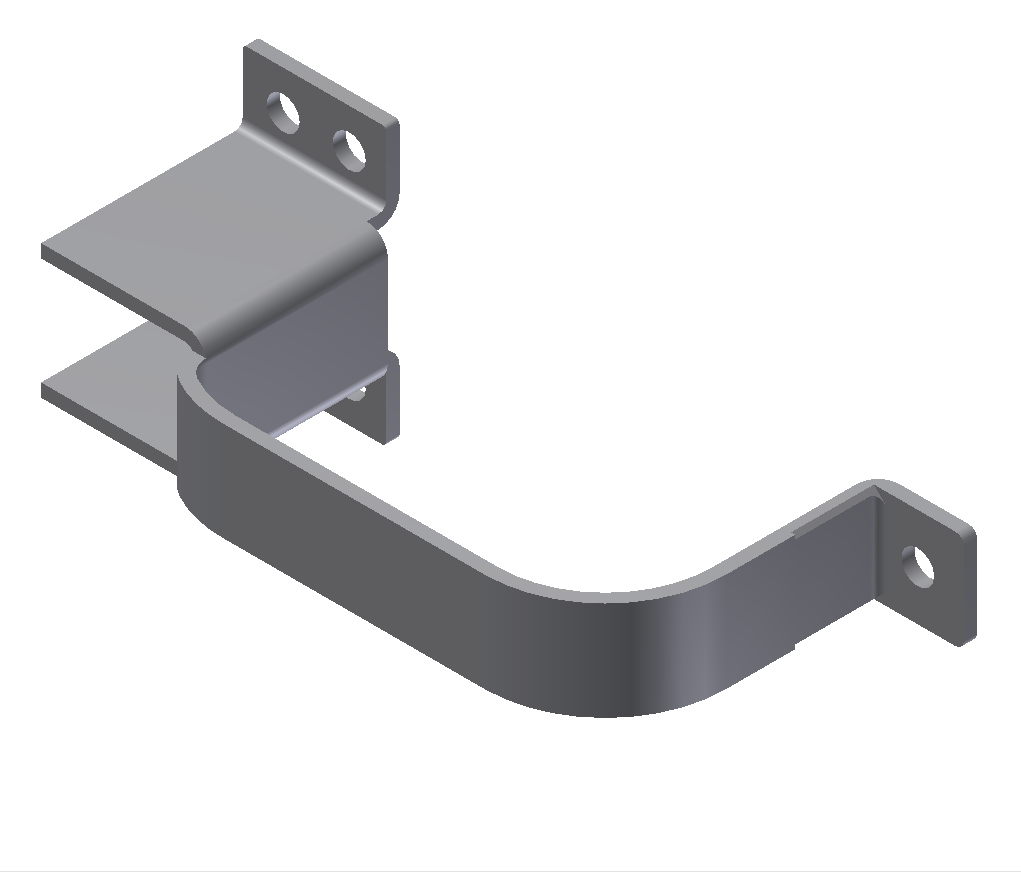
\includegraphics[width=\mymidsdormcolumnwidth\linewidth,valign=t]{../Common/images/DefeatBracketPhase_I_1}} \\
	\subfloat[Dormant Bodies piercing]{\label{fig_midsdorm}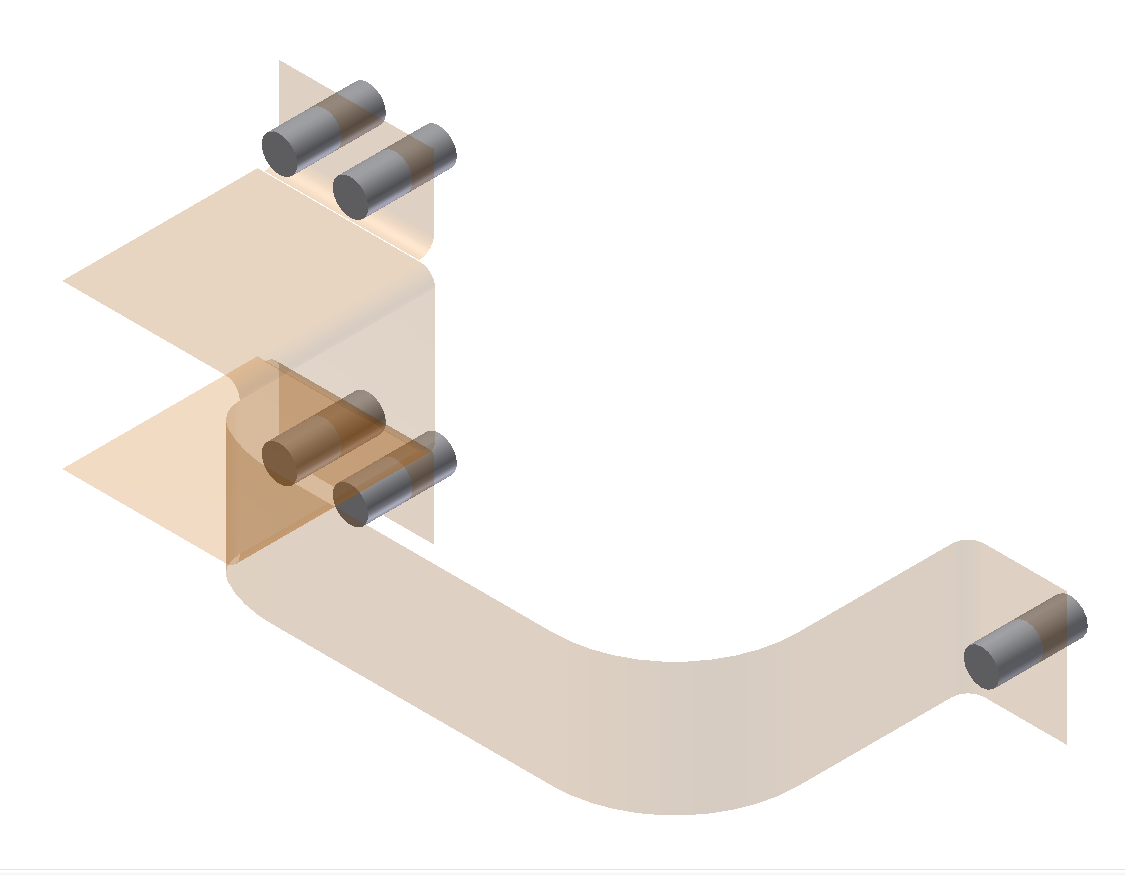
\includegraphics[width=\mymidsdormcolumnwidth\linewidth,valign=t]{../Common/images/MidsurfDormantBodies}} \qquad
	\subfloat[Final Output]{\label{fig_finalmids}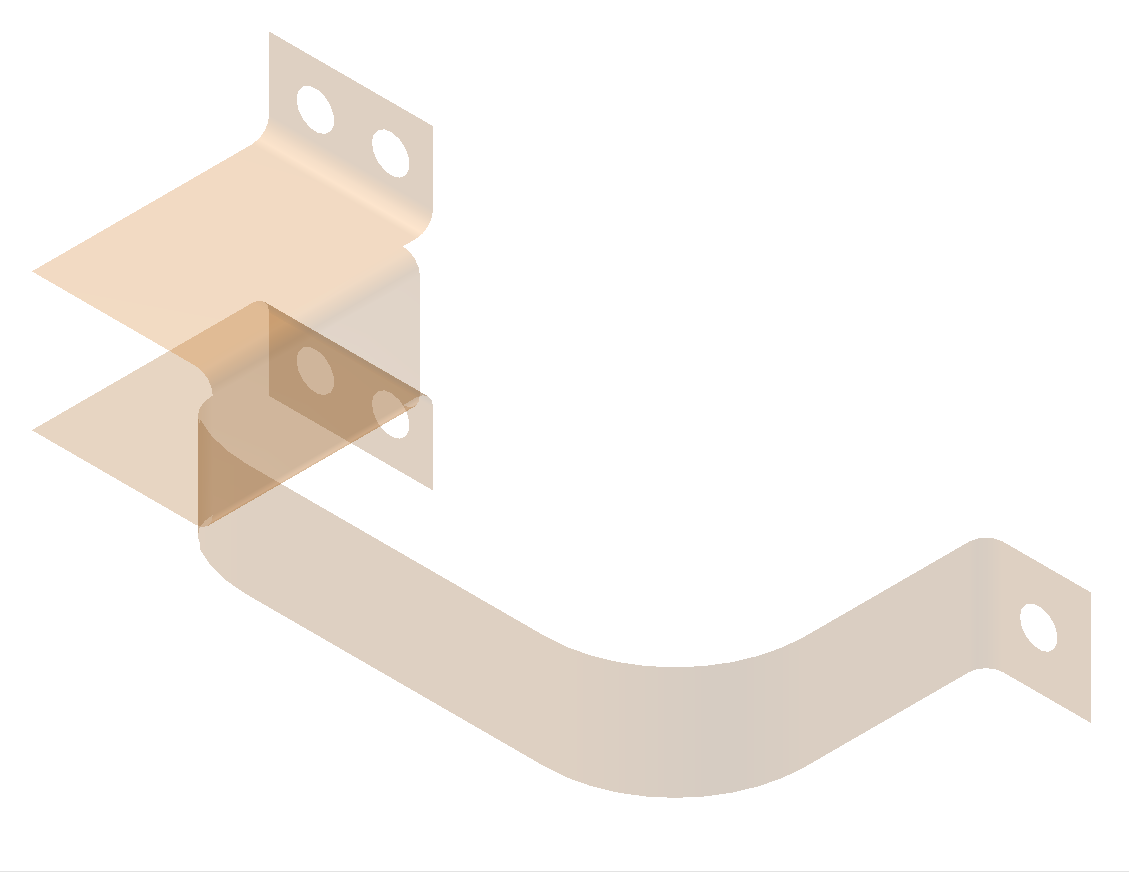
\includegraphics[width=\mymidsdormcolumnwidth\linewidth,valign=t]{../Common/images/MidsurfAfterDormant}}	
	\caption{Computation of Midsurface of a Bracket}
	\label{fig_midsdorm}
	\end{figure}

Table ~\ref{tbl_fbcm} shows various academic cases, with their respective cellular representations, graphs and midsurface outputs.

\newcommand \myColWidthFactora {0.22}
\begin{center}
\resizebox{0.6\linewidth}{!}{
%\begin{tabular}[!htb]{@{}p{0.22\linewidth} p{0.22\linewidth}  p{0.22\linewidth}  p{0.22\linewidth} @{}} \toprule
\begin{tabular}[!htb]{@{}p{\myColWidthFactora\linewidth} p{\myColWidthFactora\linewidth}  p{\myColWidthFactora\linewidth}  p{\myColWidthFactora\linewidth} @{}} \toprule
{\bf Part} & {\bf Cellular}  & {\bf Graph} & {\bf Result} \\ \midrule  

\adjustbox{valign=t}{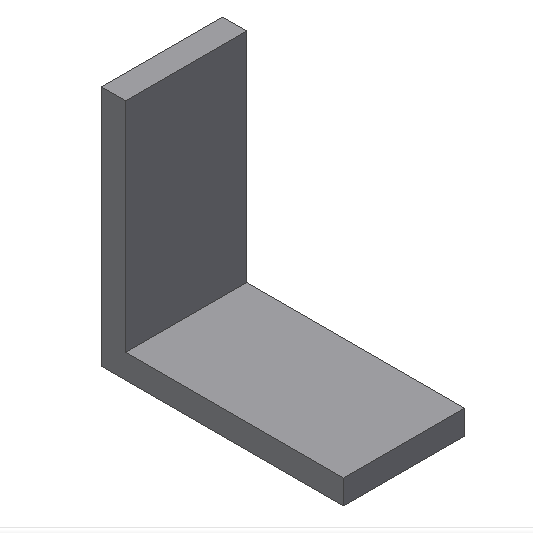
\includegraphics[width=\linewidth]{../Common/images/nonCellularL}}  &  
\adjustbox{valign=t}{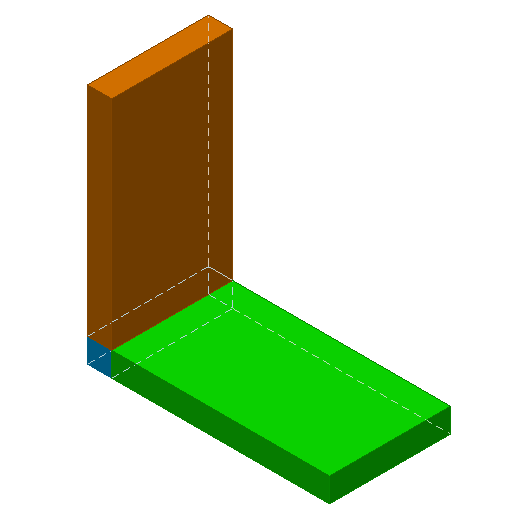
\includegraphics[width=\linewidth]{../Common/images/CellularL}}  &
\adjustbox{valign=t}{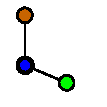
\includegraphics[width=\linewidth]{../Common/images/CellGraphL.pdf}} &  
\adjustbox{valign=t}{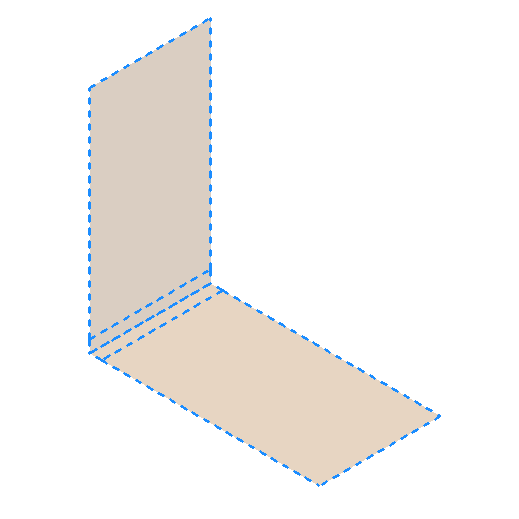
\includegraphics[width=\linewidth]{../Common/images/midsCellularL}} 
\\ \midrule

\adjustbox{valign=t}{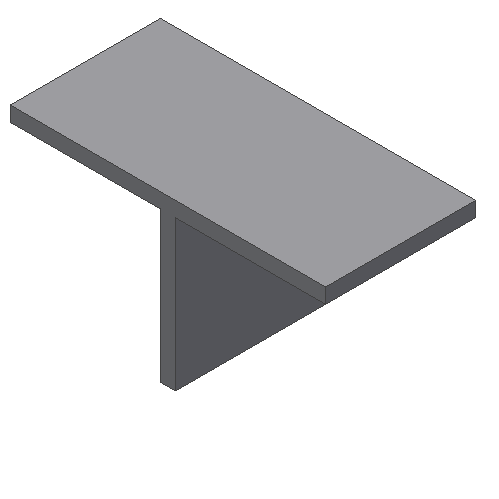
\includegraphics[width=\linewidth]{../Common/images/nonCellularT}}  &  
\adjustbox{valign=t}{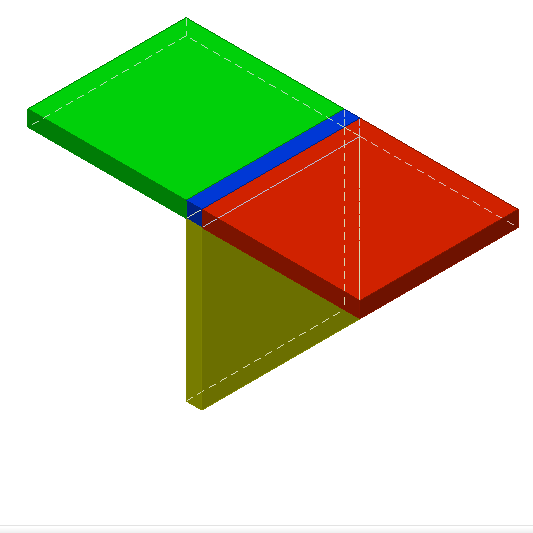
\includegraphics[width=\linewidth]{../Common/images/CellularT}}  &
\adjustbox{valign=t}{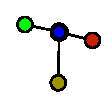
\includegraphics[width=\linewidth]{../Common/images/CellGraphT.pdf}} &  
\adjustbox{valign=t}{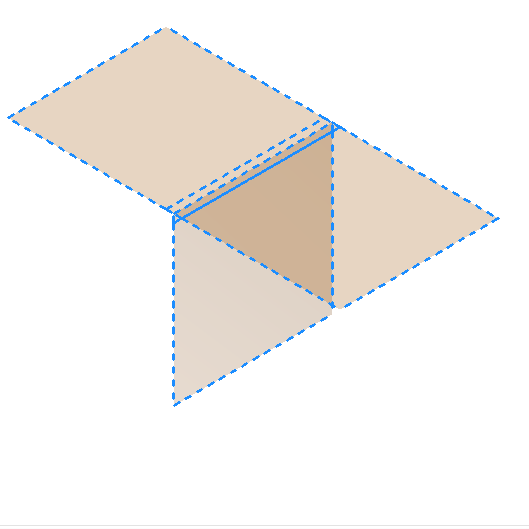
\includegraphics[width=\linewidth]{../Common/images/midsCellularT}} 
\\ \midrule

\adjustbox{valign=t}{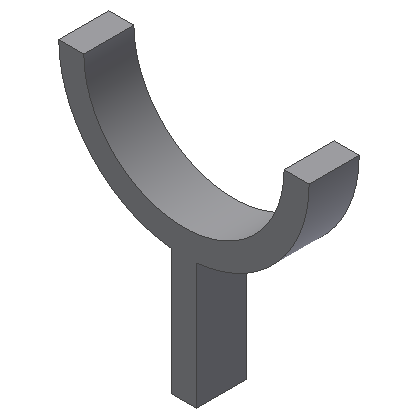
\includegraphics[width=\linewidth]{../Common/images/nonCellularCurvedY}}  &  
\adjustbox{valign=t}{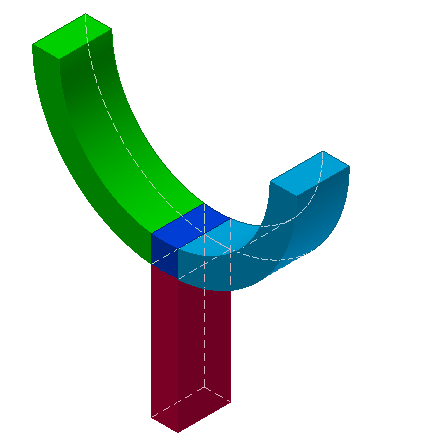
\includegraphics[width=\linewidth]{../Common/images/CellularCurvedY}}  &
\adjustbox{valign=t}{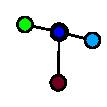
\includegraphics[width=\linewidth]{../Common/images/CellGraphY.pdf}} &  
\adjustbox{valign=t}{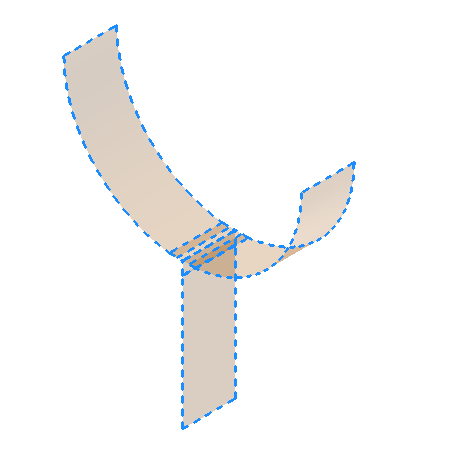
\includegraphics[width=\linewidth]{../Common/images/midsCellularCurvedY}} 
\\ \midrule

\adjustbox{valign=c}{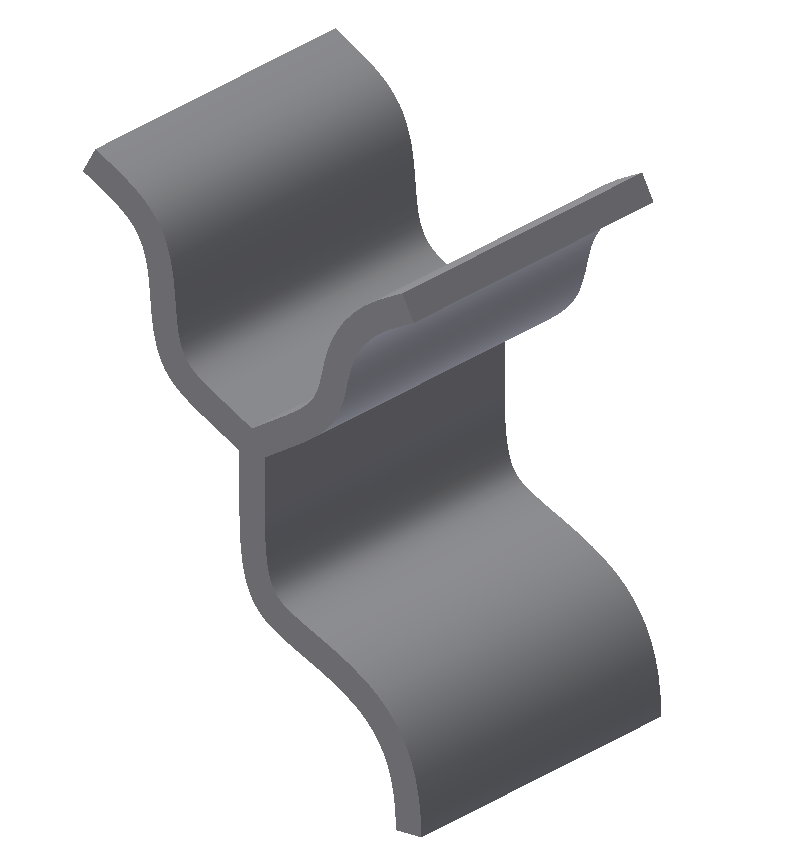
\includegraphics[width=0.8\linewidth]{../Common/images/nonCellularCurvedTri}}  &  
\adjustbox{valign=c}{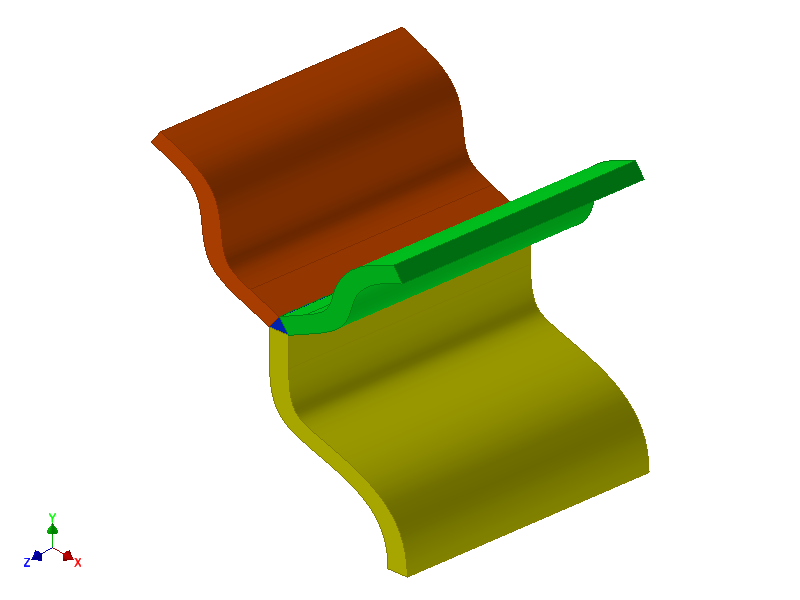
\includegraphics[width=\linewidth]{../Common/images/CellularCurvedTri}}  &
\adjustbox{valign=c}{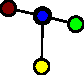
\includegraphics[width=0.8\linewidth]{../Common/images/CellGraphTri.pdf}} &  
\adjustbox{valign=c}{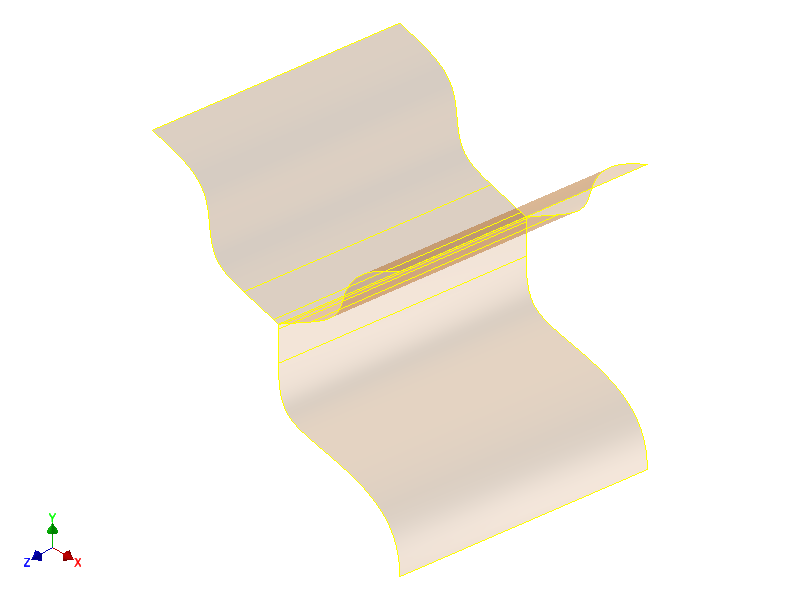
\includegraphics[width=\linewidth]{../Common/images/midsCellularCurvedTri}} 
\\ \midrule


\adjustbox{valign=t}{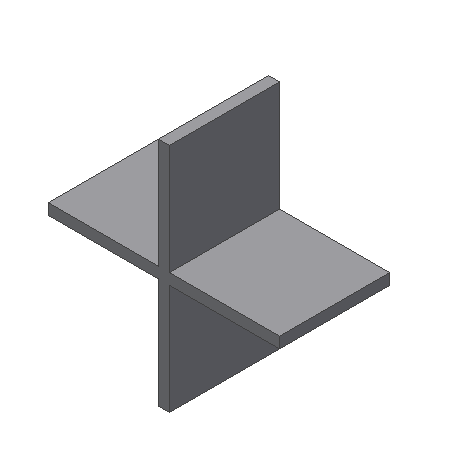
\includegraphics[width=\linewidth]{../Common/images/nonCellularPlus}}  &  
\adjustbox{valign=t}{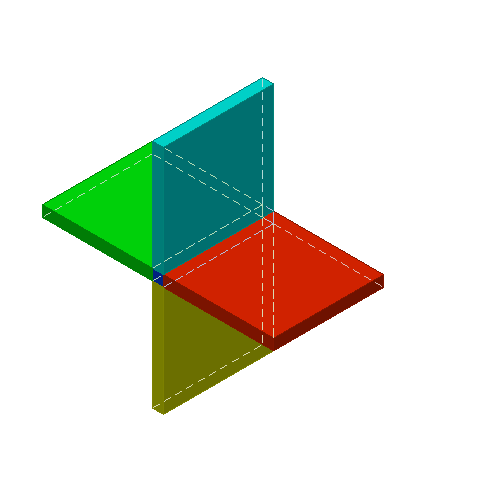
\includegraphics[width=\linewidth]{../Common/images/CellularPlus}}  &
\adjustbox{valign=t}{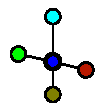
\includegraphics[width=\linewidth]{../Common/images/CellGraphPlus.pdf}} &  
\adjustbox{valign=t}{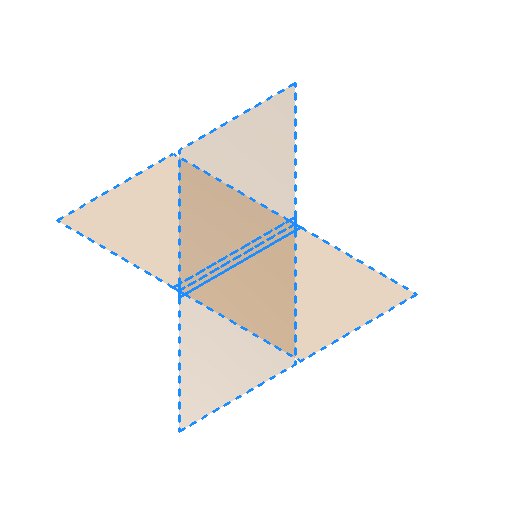
\includegraphics[width=\linewidth]{../Common/images/midsCellularPlus}} 
\\ \midrule


\adjustbox{valign=t}{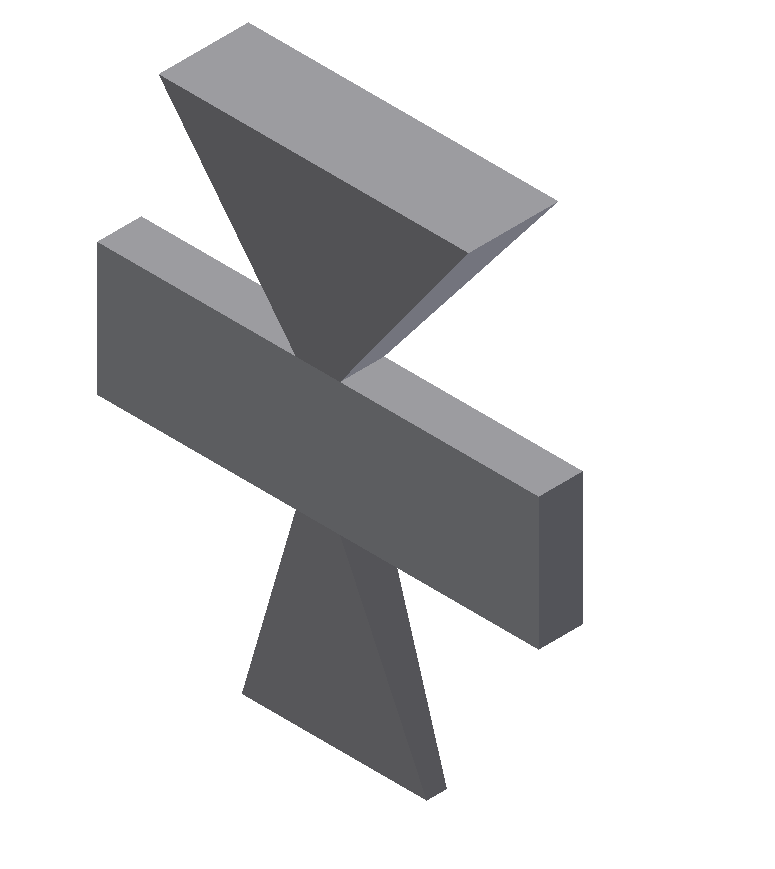
\includegraphics[width=\linewidth]{../Common/images/nonCellularDraftPlus}}  &  
\adjustbox{valign=t}{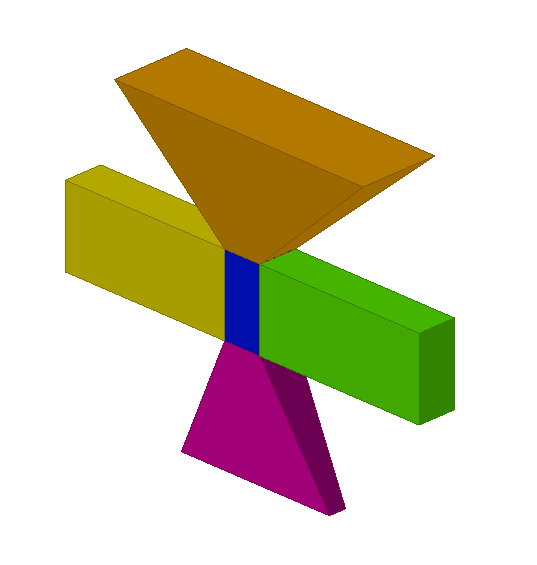
\includegraphics[width=\linewidth]{../Common/images/CellularDraftPlus}}  &
\adjustbox{valign=t}{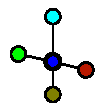
\includegraphics[width=\linewidth]{../Common/images/CellGraphPlus.pdf}} &  
\adjustbox{valign=t}{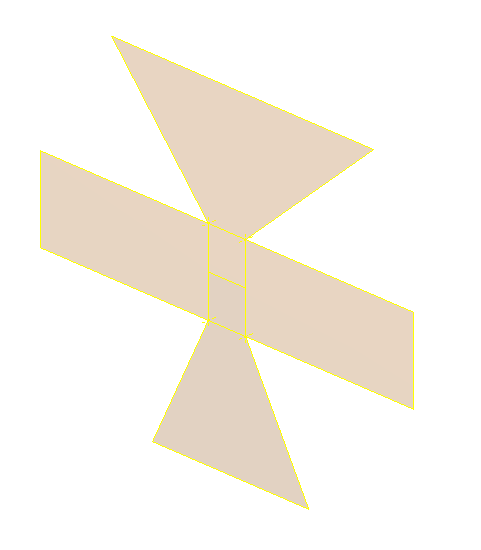
\includegraphics[width=\linewidth]{../Common/images/midsCellularDraftPlus}} 
\\ \midrule



\adjustbox{valign=t}{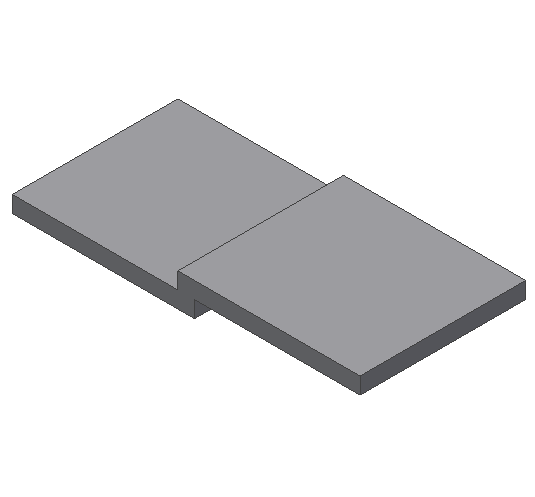
\includegraphics[width=\linewidth]{../Common/images/nonCellularOverlap}}  &  
\adjustbox{valign=t}{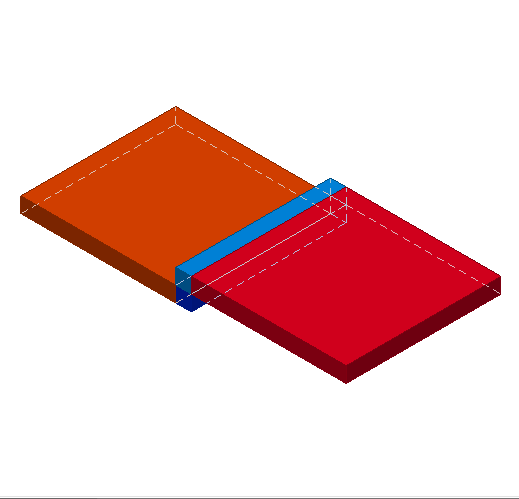
\includegraphics[width=\linewidth]{../Common/images/CellularOverlap}}  &
\adjustbox{valign=t}{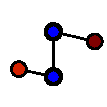
\includegraphics[width=\linewidth]{../Common/images/CellGraphOverlap.pdf}} &  
\adjustbox{valign=t}{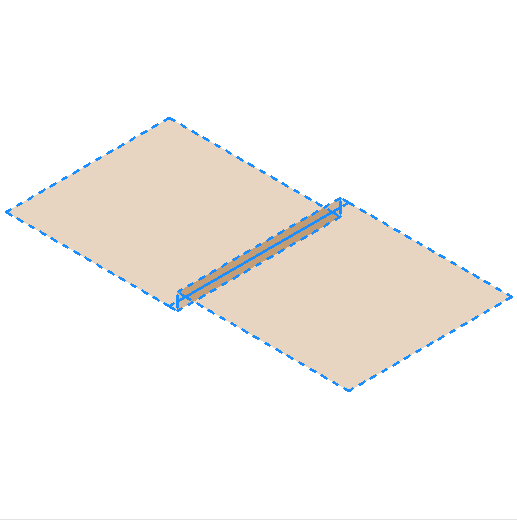
\includegraphics[width=\linewidth]{../Common/images/midsCellularOverlap}} 
\\ \midrule

\adjustbox{valign=t}{\includegraphics[width=\linewidth]{../Common/images/nonCellularZU}}  &  
\adjustbox{valign=t}{\includegraphics[width=\linewidth]{../Common/images/CellularZU}}  &
\adjustbox{valign=t}{\includegraphics[width=\linewidth]{../Common/images/CellGraphZU.pdf}} &  
\adjustbox{valign=t}{\includegraphics[width=\linewidth]{../Common/images/midsCellularZU}} 
\\ % \midrule

%\adjustbox{valign=t}{\includegraphics[width=\linewidth]{../Common/images/nonCellularBracket}}  &  
%\adjustbox{valign=t}{\includegraphics[width=\linewidth]{../Common/images/CellularBracket}}  &
%\adjustbox{valign=t}{\includegraphics[width=\linewidth]{../Common/images/CellGraphBracket.pdf}} &  
%\adjustbox{valign=t}{\includegraphics[width=\linewidth]{../Common/images/midsCellularBracket}} 
%\\ %\midrule
\bottomrule
\end{tabular}
}
\captionof{table}{Feature based Cellular Midsurface}\label{tbl_fbcm}
\end{center}
	
The superiority of the proposed approach is in the manner in which its has abstracted both the sub-problems, that is, computation of midsurface patches and resolving interactions amongst them. Hard-coded rules based on specific surface-types or connection configurations are avoided, making the whole process generic and adaptable in a wide variety of configurations.

